\chapter{Application}
In this Chapter, the data is analyzed for cointegration relations. This will first be done pair wise by use of Engel Granger. Secondly it will be for all four simultaneously with the use of Johansen test. After the models are build, they will be used for forecasts, where the predictions will be measured against the validation data to test the precision of the models.


\section{Engel Granger Model Building}
To build the models, we first check for cointegration. This is done by making a linear model of all the $12$ possible combination of the crypto currencies. In theory cointegration is not directional, but in practice one acts as the regressand and therefore we check all $12$ combinations. Hereafter it is checked whether the model is $I(0)$ which is needed for it to be cointegrated, which is done be applying the \textit{adf.test} function in \textit{R}, which calculate the augmented Dickey Fuller test, to the residuals of the model. It should be noted that the ADF's critical values are different from the normal ones used. Thus to reject the null hypothesis at a corresponding $5\%$ significance level the test statistic must be less than critical value $find hvad den skal være$. This results in the following four pair wise currencies being $I(0)$ meaning they are cointegrating. 
\pause
\begin{center}
\begin{tabular}{cccc}
   Solana \& Ethereum \quad & \quad Ripple \& Ethereum\\\\
   Ethereum \& Solana \quad & \quad Ripple \& Solana
\end{tabular}
\end{center}
\pause
\noindent The four cases will be abbreviated, SOL\&ETH, XRP\&ETH, ETH\&SOL and XRP\&SOL respectively. Next four VECM Models will be built using the above relations. First the function \textit{Varselect} is used to find the optimal lag order, the function evaluates it based on four criterions namely, Akaike Information Criterion, Hannan Quinn Criterion, Schwarz Criterion and Final prediction error. We have chosen to use AIC, since it theoretical is the best when predicting in the short term. The AIC scores for each combination have been plotted in Figure \ref{fig:AIC_plots}. The optimal lag order for a VAR model for each combination, is found by visual interpretation of the plots in Figure \ref{fig:AIC_plots}.
\begin{figure}[H]
  \centering
  \subfloat[][Solana \& Ethereum]{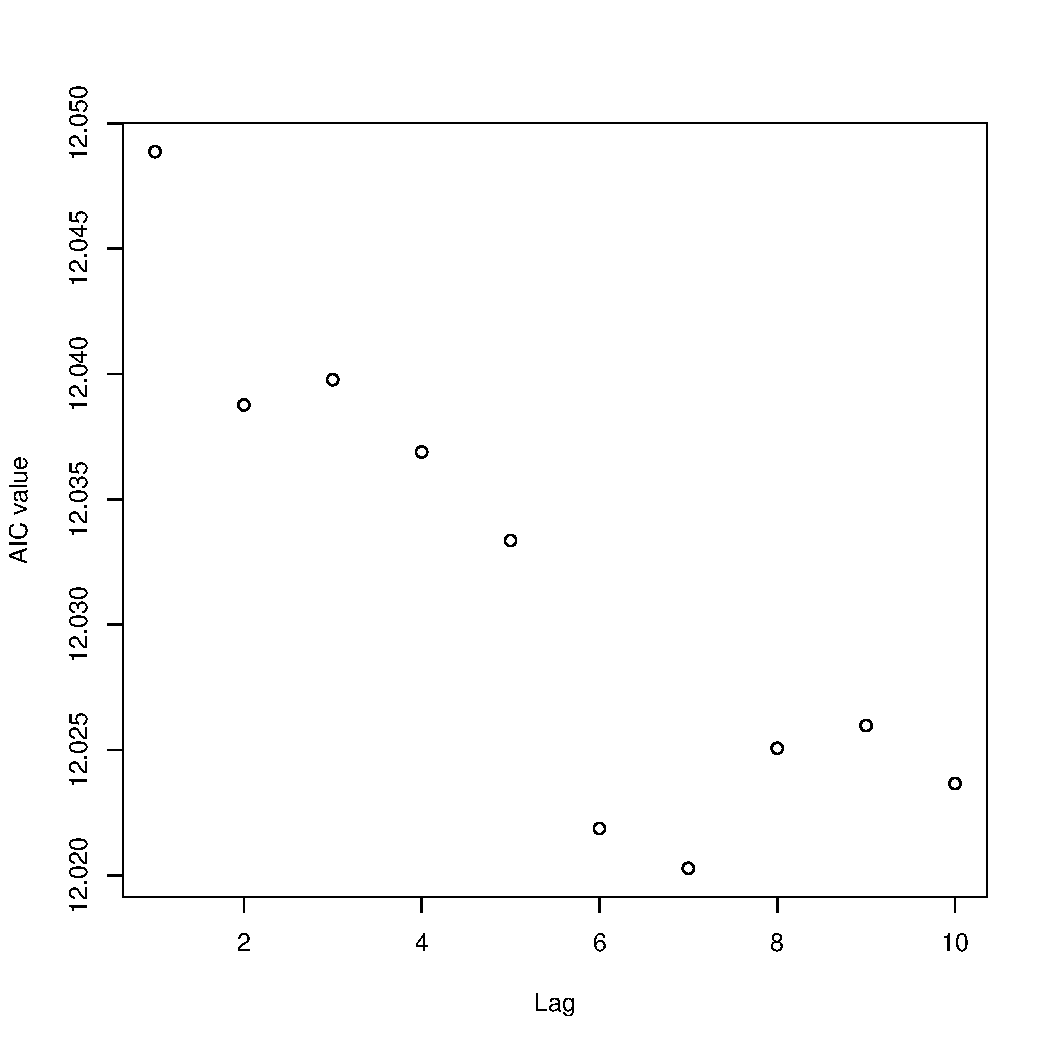
\includegraphics[width=.45\textwidth]{1.Projekt_kode/Billeder/AIC_Lag_for_SE.pdf}}\quad
  \subfloat[][Ripple \& Ethereum]{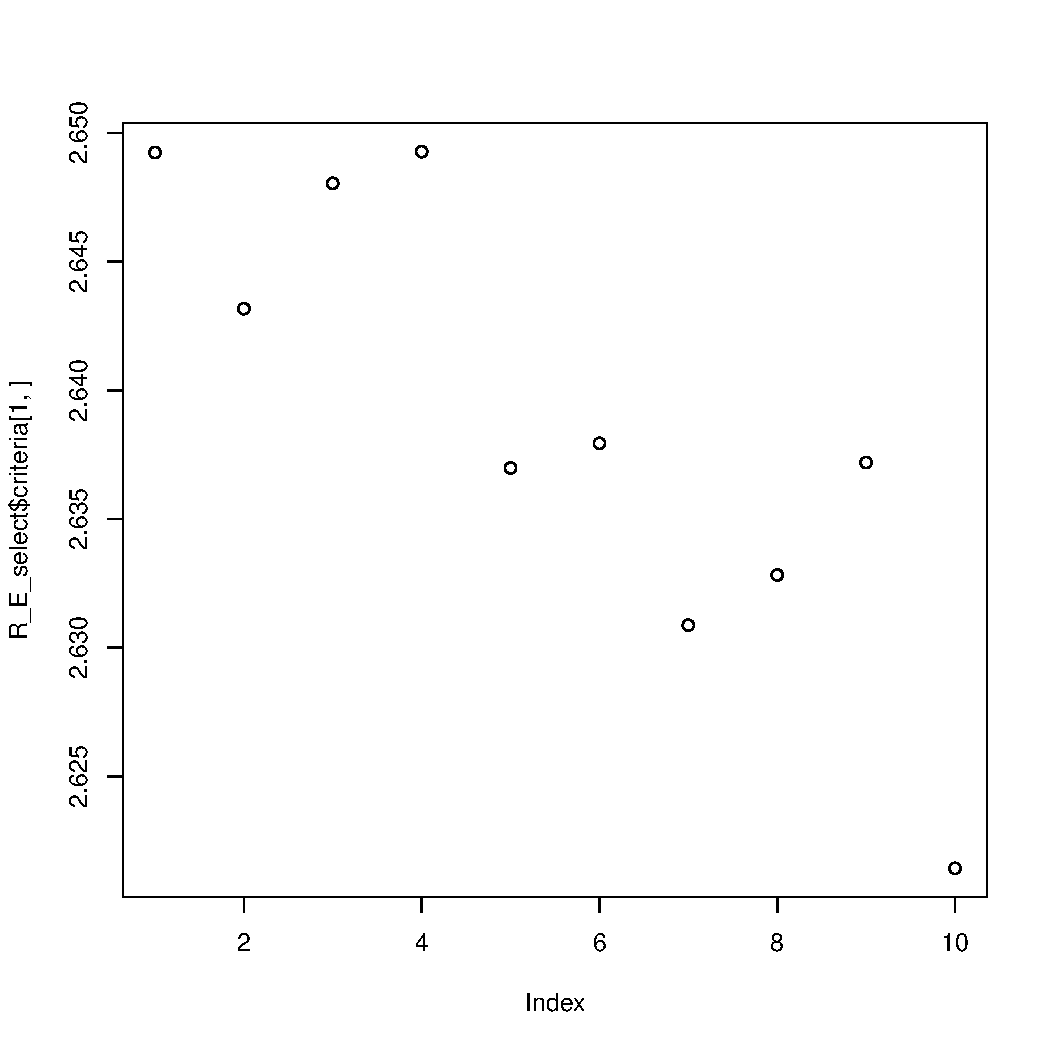
\includegraphics[width=.45\textwidth]{1.Projekt_kode/Billeder/AIC_Lag_for_RE.pdf}}\\
  \subfloat[][Ethereum \& Solana]{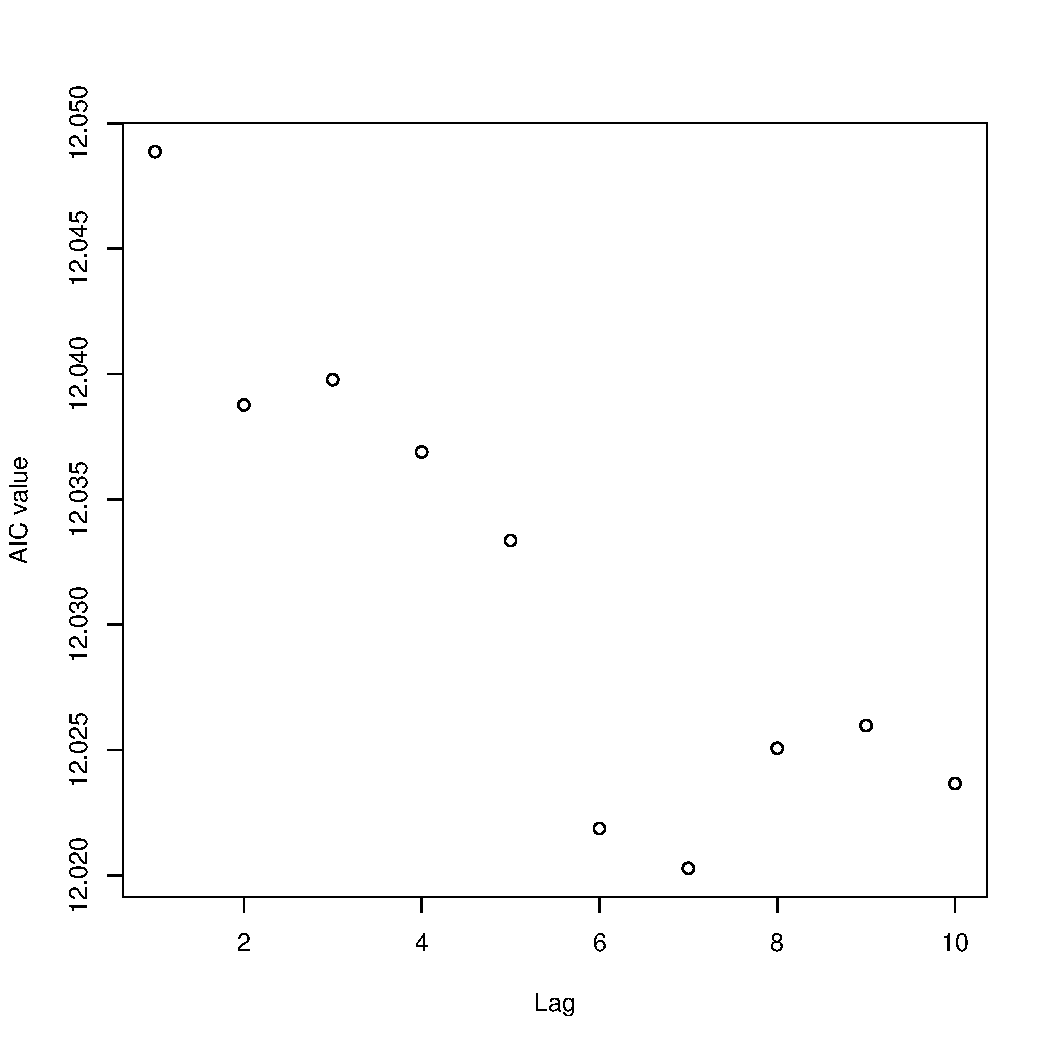
\includegraphics[width=.45\textwidth]{1.Projekt_kode/Billeder/AIC_Lag_for_ES.pdf}}\quad
  \subfloat[][Ripple \& Solana]{\includegraphics[width=.45\textwidth]{1.Projekt_kode/Billeder/AIC_Lag_for_RS.pdf}}
  \caption{AIC values for all combinations}
  \label{fig:AIC_plots}
\end{figure}
The lag order is chosen to be $VAR(6)$, $VAR(10)$, $VAR(6)$ and $VAR(6)$ respectively for each case. With the lag order determined. We can now build the VECM, where the lag order is simply one less than the $VAR$ counterpart.

The VECM is specified as follows, represented as a system of equations:\\

\begin{center}
    \textbf{SOL \& ETH}
\end{center}
$\text{Cointegrating Equation:} \quad  \beta = 1, \quad -0.03250492 \cdot \text{Ethereum} \\
\text{Equations:}$
\begin{align*}
\Delta S_t &= -0.0073 \cdot ECT_{t-1} + 0.0438 \cdot S_{t-1} - 0.0325 \cdot E_{t-1} - 0.0151 \cdot S_{t-2} - 0.0961 \cdot E_{t-2} + \dots + \varepsilon_{S_t} \\
\Delta E_t &= -0.0516 \cdot ECT_{t-1} - 1.6153 \cdot E_{t-1} + 1.8980 \cdot E_{t-4} + \dots + \varepsilon_{E_t} \\
ECT_{t-1} &= S_{t-1} - 0.0325 \cdot E_{t-1}
\end{align*}
%
\begin{center}
    \textbf{XRP \& ETH}
\end{center}
$\text{Cointegrating Equation:} \quad  \beta = 1, \quad -0.000267678 \cdot \text{Ethereum} \\
\text{Equations:} $


%
\begin{center}
   \textbf{ETH \& SOL}
\end{center}
$\text{Cointegrating Equation:} \quad  \beta = 1, \quad -25.22835 \cdot \text{Solana} \\
\text{Equations:} $


%
\begin{center}
    \textbf{XRP \& SOL}
\end{center}
$\text{Cointegrating Equation:} \quad  \beta = 1, \quad -0.006285195 \cdot \text{Solana}\\
\text{Equations:} $


%

Where:
\begin{itemize}
    \item \(\Delta \text{Solana}_t\) and \(\Delta \text{Ethereum}_t\) represent the differenced series.
    \item \(\text{ECT}_{t-1}\) is the error correction term, representing deviations from the long-term equilibrium:
    \[
    \text{ECT}_{t-1} = \text{Solana}_{t-1} - 0.0325 \cdot \text{Ethereum}_{t-1}
    \]
    \item Coefficients are reported with their corresponding standard errors (not shown for clarity here).
    \item \(\epsilon_{\text{Solana}, t}\) and \(\epsilon_{\text{Ethereum}, t}\) are error terms.
\end{itemize}

Beta coefficients for the four models:
\begin{table}[]
    \centering
    \begin{tabular}{c|c|c}
       & SE & (1, -0.03250492) \\
       &  & 
    \end{tabular}
    \caption{Caption}
    \label{tab:my_label}
\end{table}  




\section{Johansen Model Building}
One of the advantages using the Johansen test, is its ability to detect cointegration among multiple time series at a time. This means that we are not only able to look at pairwise integrated series. We will throughout this secction both be using the trace test statistic explained in Section \cite{Johansen_test} and the Maximal Eigenvalue test. \\\\
The overall difference between the two tests is that the Trace test tests has $H_0$ saying there are at max $r$ cointegration relations versus $H_1$ stating the presence of more than $r$ cointegrating relations and has the statistic described in Section \cite{Johansen_test} \eqref{eq:lrmax_coint_r} where the Maximal Eigenvalue test has $H_0$ stating the presence of $r$ cointegrating relations whereas $H_1$ indicates the presence of $r+1$ cointegrating relations and has the test statistic $-Tln(1-\lambda_{r_0+1})$ meaning it tests each eigenvalue's influence individually.\\
Generally there is little to no difference between the results achieved through the two tests. The Trace test although are more likely to dismiss $H_0$ even though it might be true hence having higher probability of type 1 errors. At the same time the Trace test is more efficient in finding cointegration relations when they do exist and is more advantageous when multiple cointegration relations exists. Since both tests are beneficial in different scenarios it is preferable to perform both to see whether the comply with each other, and if not, examine further why this could be the case \citep{johansentestdifferences}.\\\\

\subsection{Trace test}
From earlier 




\section{Forecast}
To evaluate models ability to correctly forecast, we first look at a plot of a single 20-day-ahead prediction. Secondly an 5-day-ahead forecast has been made iteratively, with each iteration adding another day to the training data set until the entire validation data set has been predicted upon. These predictions will be evaluated using the three different means mean absolute value, root mean square error and mean absolute percentage error:
\begin{align*}
    \text{MAE} = \frac{1}{n} \sum_{i=1}^{n} |y_i - \hat{y}_i|, \quad \text{RMSE} = \sqrt{\frac{1}{n} \sum_{i=1}^{n} (y_i - \hat{y}_i)^2}, \quad \text{MAPE} = \frac{1}{n} \sum_{i=1}^{n} \left| \frac{y_i - \hat{y}_i}{y_i} \right| \times 100
\end{align*}
\textbf{Engel Granger}

\begin{figure}
    \centering
    \includegraphics[width=0.5\linewidth]{}
    \caption{Caption}
    \label{fig:enter-label}
\end{figure}